\chapter{Arbiter \acsp{PUF}}
\label{cap:arbiter}

\apufs were introduced already in 2002 as new delay-based \puf \cite{Gassend2002SiliconFunctions}.
Over the year 2016 they got more attention, since their implementation is resource-efficient and low cost \cite{Becker2014ActiveDesigns,Suh2007PhysicalGeneration}.
However, there are still challenges due to the security concerns of classic \apufs, as described in Sec.\ \ref{sec:attacksonarbiter} \cite{Ganji2016PACPUFs, Ruhrmair2014PUFOverview}.

The relatively simple design, compared to e.g.\ cellular nonlinear network \pufs, of \apufs makes it appealing to people to seek new improved possible varieties including the popular \xpuf, which will be presented in this section. %+
% Due to new problems which occur with the design improvement of \xpufs it is impossible to realize them securely.
Due to challenges, which occur when combining a large amount of \apufs to a \xpufs, it is so far impossible to realize large \xpufs \cite{Rostami2014RobustMatching}.

% old: Further, the success of attacks on \xpufs depends on their size, it is also not possible to build \xpufs that are secure and usable \cite{Ganji2015WhyPUFs}. %+
Furthermore, the success of attacks on \xpufs depends on their size and as there is a limit it is also not possible to build \xpufs that are secure and usable \cite{Ganji2015WhyPUFs}. %+
For these reasons there is still further improvement needed to call \apufs to be practically secure, even for enhanced versions like for example \xpufs.
That is why I chose to study \apufs and \xpufs instead of other types of \pufs introduced in Sec.\ \ref{sec:typesofpufs} in this thesis.

This sections starts with a description of how \apufs work and the differences of \xpufs.
Subsequently, two models are explained. %+
The first one gives an introduction on how \apufs can be physically built.
The second one defines the theoretical models of \apufs used to attack them later in this thesis.

\section{\apufs}
\label{sec:arbiter}

The concept of an \apufs is based on the difference of the delays of two signals, which gets converted to a single bit response. 
To implement this concept, an \apuf has multiple connected stages and an arbiter at the end, as shown in Fig.\ \ref{fig:arbiter}.

Both signals propagate on parallel paths with the same layout length through all stages until they reach the arbiter.
The arbiter then outputs the response bit depending on which input of the arbiter is triggered first by one of the signals. %+
Every stage has three inputs, two for both signals and one for one bit of the challenge.
This challenge bit determines if the signal paths will be crossed in this stage. %+
If the bit is 0, both signals will flow parallel through the stage.
If the bit is 1, the stage will swap the signal flow.
So the paths for the signals through the stages exclusively depends on the challenge $\gls{c} = (c_1, c_2, \cdots, c_n)$.

\begin{figure}[ht]
\centering
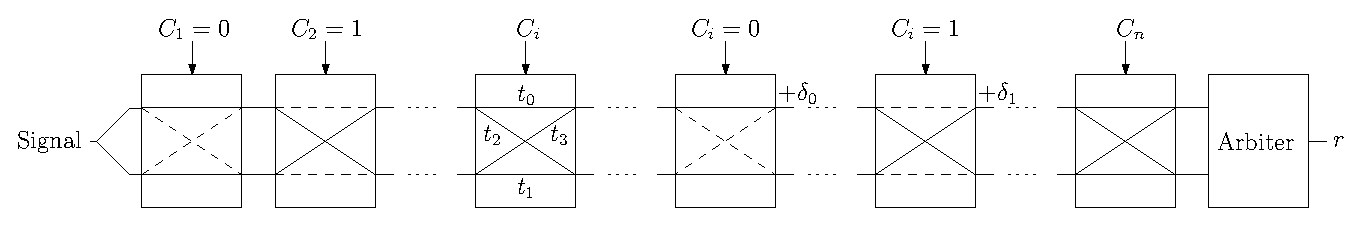
\includegraphics[width=1.00\textwidth]{images/arbiter_puf.eps}
% \noindent\includegraphics[width=1.00\textwidth, height=3cm, draft]{example-image-a}
\caption{\apuf}
\label{fig:arbiter}
\end{figure}

The challenge bit length must match the number of stages in the \apuf so every stage gets a challenge bit assigned. 
This is called the size $\gls{n}$ of the \apuf in this work. %+
The circuits of both paths are laid out to have logical equal length.
% "Although the circuit is laid out to have equal length on all paths, any physical realization will have different signal delays that are due to chip imperfections."
But, due to the inaccuracies in the manufacturing process of the electronic devices used for the stages, which can not be influenced by the producer, transit times will differ from device to device.
These differences can be seen as the intrinsic unique key of an instance of every \apuf. %+
One stage for itself has 4 different signal paths: 

\begin{itemize}
\item top input - top output: $\gls{t}_0$
\item bottom input - bottom output: $\gls{t}_1$
\item top input - bottom output: $\gls{t}_2$
\item bottom input - top output: $\gls{t}_3$
\end{itemize}

Nevertheless, there are just two combinations possible, as the stage input is a Boolean value.
Either its top input to top output and bottom output to bottom output or its top input to bottom output and bottom input to top output.
These combinations lead to the delay differences $\gls{t}_0 - \gls{t}_1 = \delta_0$ and $\gls{t}_2 - \gls{t}_3 = \delta_1$ for the possible input 0 or 1 per stage. %+
Additional, to the delay differences, which remain constant, deviations are occurring during the \apuf is queried.
These deviations are noise and one way to model them is to use two distinct random variables.
Both variables are normally distributed with mean zero and can be described as follows:

\begin{itemize}
\item At every stage of the \apuf, additionally to the chosen delay differences $\delta_0$ or $\delta_1$, normally distributed noise with zero mean and give variance occurs.
\item At the arbiter normally distributed noise with zero mean and given variance leads to a different output of the comparison sometimes.
\end{itemize}

% This internal noise leads to a certain amount of so called ‘‘unstable’’ challenges for a specific \apuf. 
% Unstable challenges tend to lead to different responses when evaluating multiple times.
Due to the internal noise, the PUF may return different responses when given the same challenges twice.
That is because challenges in combination with the different path delay values can result in a very small difference between the appearing signals on the arbiter. %+
This small difference can be changed by the introduced noise or the arbiter can decide wrong due to its own noise every time the \apuf is queried and so the final response can be changed. %+

Hence, every challenge has its own stability value, which is defined in Eq.\ (\ref{equ:stability}), and challenges with a lower stability value are called unstable.
Whether a challenge is called unstable, depends on its stability value and the limit within a challenge is defined as stable.
This limit is not generally defined and can be set as needed.
Is the stability value below this limit the challenge is called unstable.

These are all parts to evaluate and to specify an \apuf.
The \xpuf, which is based on \apufs, will be outlined in Sec.\ \ref{sec:xorarbiterpufs}.
One way how an \apuf can be built and its possible internal structure will be presented in Sec.\ \ref{sec:physical}.
%A more detailed description how it is build and what the physical features are will be presented in Sec.\ \ref{sec:physical}.
The theoretical characterizations, a prerequisite for attacks, are part of Sec.\ \ref{sec:theoretical}.
Successful attacks on \apufs have been already developed and will be mentioned in Sec.\ \ref{sec:attacksonarbiter}.

%========================================
% n restriction by the size of the chip or costs \cite{Ganji2015WhyPUFs}

\section{\acs{XOR} \apufs}
\label{sec:xorarbiterpufs}

The \xpuf is one attempt to improve the security of \apufs and has been proposed by Suh and Devadas in 2007 \cite{Suh2007PhysicalGeneration}.
It combines multiple individual \apufs with an \acf{XOR} function to a \xpuf, as shown in Fig.\ \ref{fig:xorarbiter}.

As the \ac{XOR} function is not a linear separable function, as defined in Chap.\ \ref{cap:mla}, it adds non-linearity to the \puf. 
% https://en.wikipedia.org/wiki/Exclusive_or
% https://www.quora.com/Why-cant-the-XOR-problem-be-solved-by-a-one-layer-perceptron
This non-linearity increases the effort on the side of the attacker and makes machine learning attacks more difficult \cite{Becker2010OnBifurcation, Lim2005ExtractingCircuits}.
% This non-linearity increases the complexity to make machine learning attacks more difficult since we can not prevent them \cite{Greibach2010OnBifurcation, Lim2005ExtractingCircuits}.
Another approach to add non-linearity are Feed-forward \apufs proposed by Lim et al.\ \cite{Lim2005ExtractingCircuits}.

\begin{figure}[ht]
\centering
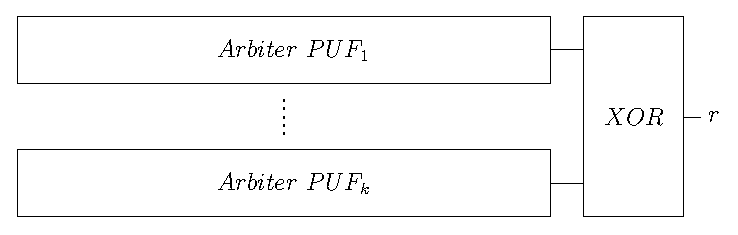
\includegraphics[width=1.00\textwidth]{images/xor_arbiter.eps}
% \noindent\includegraphics[width=1.00\textwidth, height=3cm, draft]{example-image-a}
\caption[\acs{XOR} \apuf]{\xpuf}
\label{fig:xorarbiter}
\end{figure}

Every \apuf operates in the manner of the characterization in Sec.\ \ref{sec:arbiter}. 
To improve the security the \ac{XOR} function adds up all responses to hide the response of every single \apuf instance.
If the attacker does not know the response of a single \apuf, he will not be able to separately attack every single \apuf of the \xpuf \cite{Becker2015ThePUFs}. %+
% This protects the underling \apufs against direct attacks and if there are no more information revealed, e.g.\ though side channel attacks as described in Sec.\ \ref{sec:attacksonarbiter}, the attacker has to model the whole \xpuf to be successful.
This protects the underling \apufs against direct attacks and under the condition that there are no more information revealed, through e.g.\ side channel attacks, as mentioned in Sec.\ \ref{sec:attacksonarbiter}, the attacker has to model the complete \xpuf at once to be successful.


The number of combined \apufs $\gls{k}$ has the following two impacts on the \puf.
Using more \apufs increases the resistance against modeling attacks, but also decreases the stability, which makes the \puf less reliable \cite{Becker2015ThePUFs, Ganji2015WhyPUFs}. %+
Stability here means the likelihood that the \apuf responses equally to an \apuf with the same internal values but without noise when processing the same challenge under the same environmental conditions. %+
% This opposed relation between stability and number of \apufs is due the fact that the errors are amplified by the \ac{XOR} function which leads to a maximum in the number of used \apufs for real applications \cite{Rostami2014RobustMatching}.

The decrease of the stability of the entire \xpuf caused by using more \apufs is due the fact that the less stable challenges of every \apuf are accumulated by the \ac{XOR} function \cite{Rostami2014RobustMatching}.
That leads to a maximum in the number of used \apufs for real applications, since they have to meet a certain stability for a reliable repeatability \cite{Rostami2014RobustMatching}.

The stability of an \apuf designed on a 65 nm technology is supposed to be $96\ \%$ \cite{Rostami2014RobustMatching}.
This relation between the production technology and the stability, as Rostami et al.\ mentioned, is not part of this work and will therefore not be further studied \cite{Rostami2014RobustMatching}. %+
Using $12$ \apufs in a \xpuf leads to a total stability of approximately $50\ \%$, as the noise of $4\ \%$ of every \apuf gets added up and is not usable, since the response is not stable reproducible, as Ganji et al.\ implied \cite{Ganji2015WhyPUFs}. %+

Yet Yu et al.\ suggested that the accumulation of the \apuf noise values to obtain the \xpuf noise value, done by Ganji et al.\, is not precise enough.
Accordingly, the stability of a \xpuf with $\gls{k} = 12$ is $67\ \%$ for an even lower stability of $95.7\ \%$ for the included \apufs \cite{Yu2016AAuthentication}. %+
% Considering that, if there exists a limit for size $\gls{k}$ of a \xpuf, it will depend on the required stability and the stability of the used \apufs.
Considering that, the limit for size $\gls{k}$ of a \xpuf depends on the required stability and the stability of the used \apufs.

The size of the challenge of a \xpuf is the same as the size $\gls{n}$ of the underlying \apufs.
All internal \apufs have the same size.
The challenge must be distributed to all internal \apufs. %+
The approach for \xpufs is to apply the same challenge to every \apuf.
For the reason to make machine learning attacks more difficult, it is suggested to apply different challenges to every \apuf. %+

However, applying a more large challenge of size $\gls{n} \cdot \gls{k}$ to the \xpuf and then distributing individual challenges of size $\gls{n}$ to every \apuf reopens possibilities to directly attack individual \apufs by changing only their challenge fraction \cite{Becker2015ThePUFs}.

Another way is to shift the challenge depending on the size of the \puf and the number of \apufs every time before it will be applied to the next \apuf.
Thus, in the best case every challenge bit takes every place in the challenge once when getting applied to different \apufs. %+
It is so far unproved that each input bit of an \apuf has a different high likelihood to affect the response.
But, by transforming the challenge in this way, the likelihood of every bit to affect the response becomes more balanced, which makes the \puf less predictable and more difficult to attack.

As this challenge transformation is part of Lightweight \pufs, it will not be part of this work.
For more detailed information I refer the reader to Majzoobi et al.\ \cite{Majzoobi2008LightweightPUFs}.

%========================================
% Further points
% Difference between arbiter puf and xor arbiter puf?
% Why attackers win: On the learnability of XOR arbiter PUFs: LTF Darstellung
% Warum Stage Distribution und Noice etc: Seite 15 unten \cite{Becker2015ThePUFs}
% k restriction by the size of the chip or costs
% the number of noisy response of an XOR PUF is virtually equal to the sum of the number of noisy response of each individual arbiter PUF [21]. In the literature majority voting is suggested as a solution to deal with noisy responses [18,23]. \cite{Ganji2015WhyPUFs}
% large XOR Arbiter PUFs are infeasible to build, as their stability will decrease exponentially with growing k [8]. Why-Attackers-Lose

\section{Model}
\label{sec:model}

An \apuf and so its intrinsic secret can be manifested in different ways.
% In this work the physical model and theoretical model are studied. %+
The following section explains a physical implementation of \apufs to provide an insight of \apuf implementations for real purpose. %+

Furthermore, the theoretical models of \apufs are defined, since they are used by the simulation of \apufs.
They serve also as representation for the results of attacks stated in Sec.\ \ref{cap:mla}.
This representation is not unclonable, as the values of the theoretical model are exposed and can be duplicated.

% old:
% The physical model is the description how \apufs can be built to use them for real purpose.
% The theoretical model represents an \apuf and is used for simulations.
% It serves thus as representation used as result of attacks explained in Sec.\ \ref{cap:mla}.
% This representation is not unclonable as the values of the theoretical model are exposed and can be duplicated.

\subsection{Physical}
\label{sec:physical}

For real world use cases \apufs have to be built as circuits to include them into devices.
There are different possible engineering techniques to realize them.
An \ac{ASIC}, \ac{FPGA} or \ac{CPLD} are the most common ones \cite{Maes2012ExperimentalCMOS, Majzoobi2010FPGALines, Soybali2011ImplementationFPGA, Tajik2014PhysicalPUFs}.

The solution provided by an \ac{ASIC} fits the logical layout of an \apuf best and is therefore the most accurate one. %+
Yet for development purpose this technique is very expensive.
Every time the layout changes a new wafer as core of an \ac{ASIC} has to be produced.
This manufacturing process is very costly and mainly used for the final product.
Consequently, \ac{ASIC} are used when high quantities of chips is needed.

A cheaper way is to use a \ac{FPGA} or \ac{CPLD}. 
A \ac{FPGA} is a programmable \ac{IC}, which can be programmed over and over again with very little effort.
It consists of an array of \acp{CLB}, here called gates, connected through a mesh. %+
The \ac{HDL} tells the \ac{FPGA} network how to connect the gates to obtain the desired circuit behavior. %+
\ac{CPLD} follow a similar principle as the \ac{FPGA}, but are smaller in terms of resources and have a less complex structure.

Nevertheless, \ac{FPGA} suffer from different problems making it difficult to use them as secure \apuf implementation.
When describing the circuit layout of the chip with \ac{HDL}, its code has to be compiled before transferring. %+
In the compilation process the compiler determines, which physical gates on the chip will be used for the circuit design due to the specific chip type and its interconnect structure.
This defines the used circuit traces between the used gates and lead to asymmetric routes. %+ % makes exact symmetric routing in most cases not realizable.

Asymmetries in routing means that the trace to connect two gates is different in its physical length to its parallel opponent.
This can lead to bias in the mean of the distribution of the delay differences of an \apuf, explained in Sec.\ \ref{sec:arbiter}, making the responses predictable and introduces a lack of randomness \cite{Majzoobi2010FPGALines, Morozov2010AnFPGA}. %+
The variation of the traces can be even higher than the manufacturing variations of the stage implementations, so that the response is mainly decided by the routing delays instead of the different variation combination of the used stage paths \cite{Majzoobi2009TechniquesPUFs}.

To counter these problems a concept of multiple combined \apuf called Double \apuf has been suggested \cite{Machida2015ImplementationFPGA, Machida2015AFPGA}.
The \apufs, considered in this thesis, are implemented by \ac{ASIC}, as there are all necessary electronic components placed and connected freely.
Accordingly, \apuf implementations in an \ac{ASIC} will be further studied.

% old: 
% The necessary components other than the conductor paths, whose layout have to be designed symmetric and of the same capacitive loads, are implementations of the stages and the arbiter \cite{Maes2012ExperimentalCMOS}.
For \apuf implementations in an \ac{ASIC} all conductor paths have to have a symmetric layout with the same capacitive loads to prevent the named bias of the delay differences.
To implement the stages and the arbiter different electric components are required \cite{Maes2012ExperimentalCMOS}. %+
For the hardware realization of a single stage two 2-to-1 \ac{MUX} are used, as suggested by Rührmair et al.\ \cite{Ruhrmair2013PUFData, Lee2004AApplications}.%+

There are analog or digital \ac{MUX} available. %+
Their design differences lead to a greater delay in passing the signal to its output for digital \ac{MUX} compared to analog ones \cite{Mano2008Logicfundamentals}.
Additional differences, e.g.\ clipping parts of a continuous signal when exceeding a specific voltage, do not apply here, since the \apuf has only sign signals \cite{Semiconductor2002BasicComparison}. %+

The sign signal of an \apuf is the signal, which propagates through the stages of the \apuf, shown in Sec.\ \ref{sec:arbiter}.
It has two definite states, high and low, whereby high triggers the arbiter.
Other values then high and low are not definite values of the signal and not used.
% https://en.wikipedia.org/wiki/Square_wave

Hence, both types of \ac{MUX} can be used unless they get mixed.
Fig.\ \ref{fig:multiplexer} shows a single analog \ac{CMOS} \ac{MUX} and how two of them used to build a complete stage component. %+
The signals $\gls{s}_1$ and $\gls{s}_2$ are connected to the output $\gls{o}_1$ and $\gls{o}_2$ depending on the challenge bit $c_i$.
Additional, there are some buffers used in the \ac{ASIC} design, which yet are not needed for understanding.

\begin{figure}[ht]
\centering
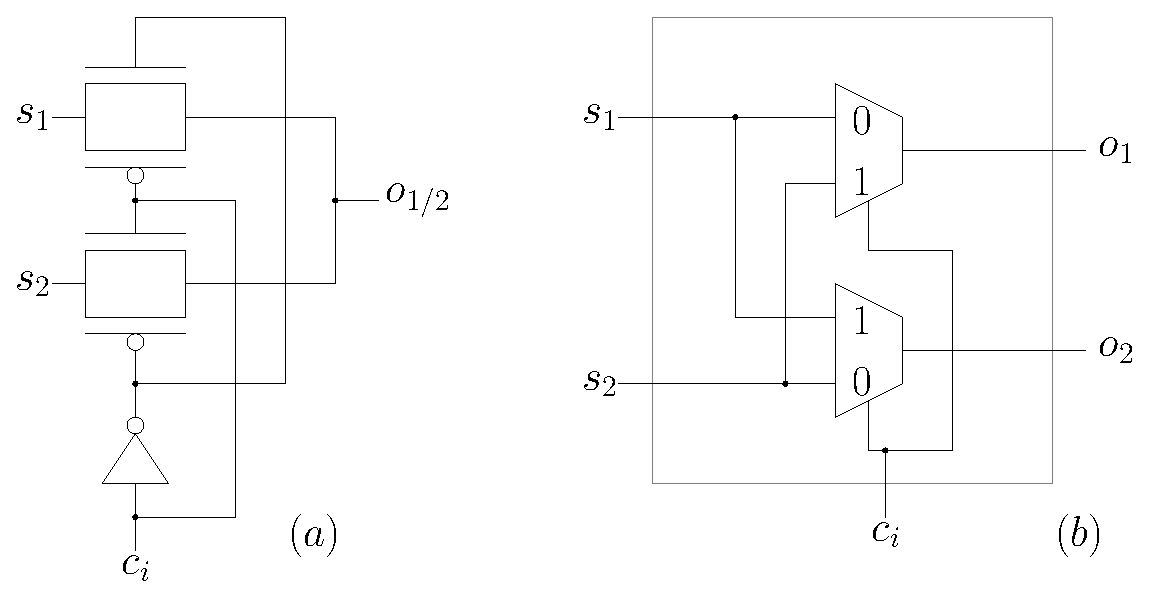
\includegraphics[width=0.70\textwidth]{images/stage_circuit.eps}
% \noindent\includegraphics[width=1.00\textwidth, height=3cm, draft]{example-image-a}
%\cite{Semiconductor2002BasicComparison}
%\cite{Lee2004AApplications}
\caption[Analog \acs{MUX} and stage circuit]{(a) Analog \ac{CMOS} \ac{MUX} realization with single output.
(b) Two \acs{MUX} connected to complete stage circuit.}
\label{fig:multiplexer}
\end{figure}

% The arbiter's task is to determine at which input of the arbiter a signal arrives first.
% The inputs of the arbiter are the same as the ends of the stage chains.
The arbiter's task is to determine, which signal arrives first at the end of the stage chain.
The ends of the stage chains are the same as the inputs of the arbiter. %+
To provide this function a \ac{SR-latch} is used that can be realized in different ways with NOR, NAND, or AND-OR logic gates \cite{Mano2008Logicfundamentals}.
Using NAND logic gates is the method of choice, since it has a symmetric construction and because of that it is unbiased \cite{Lin2010Low-powerFunctions,Maes2013PhysicallyApplications}.

Fig.\ \ref{fig:nandarbiter} displays the switching circuit built with two cross-coupled \ac{CMOS} NAND gates for an arbiter \cite{Mano2008Logicfundamentals}.
The internal states of the outputs $r$ and $rb$ are initial high. 
A rising edge of a signal occurring on $\gls{s}_1$ will pull down $r$ and the other way round.
The output states low or high are equal to the response values of the \puf $0$ or $1$. %+
Ensured by the cross-coupling, only one competing transition can win and the symmetric layout prevents circuit design based bias.
NOR logic gates could be used likewise, as their \ac{SR-latch} implementation is also symmetric.

\begin{figure}[ht]
\centering
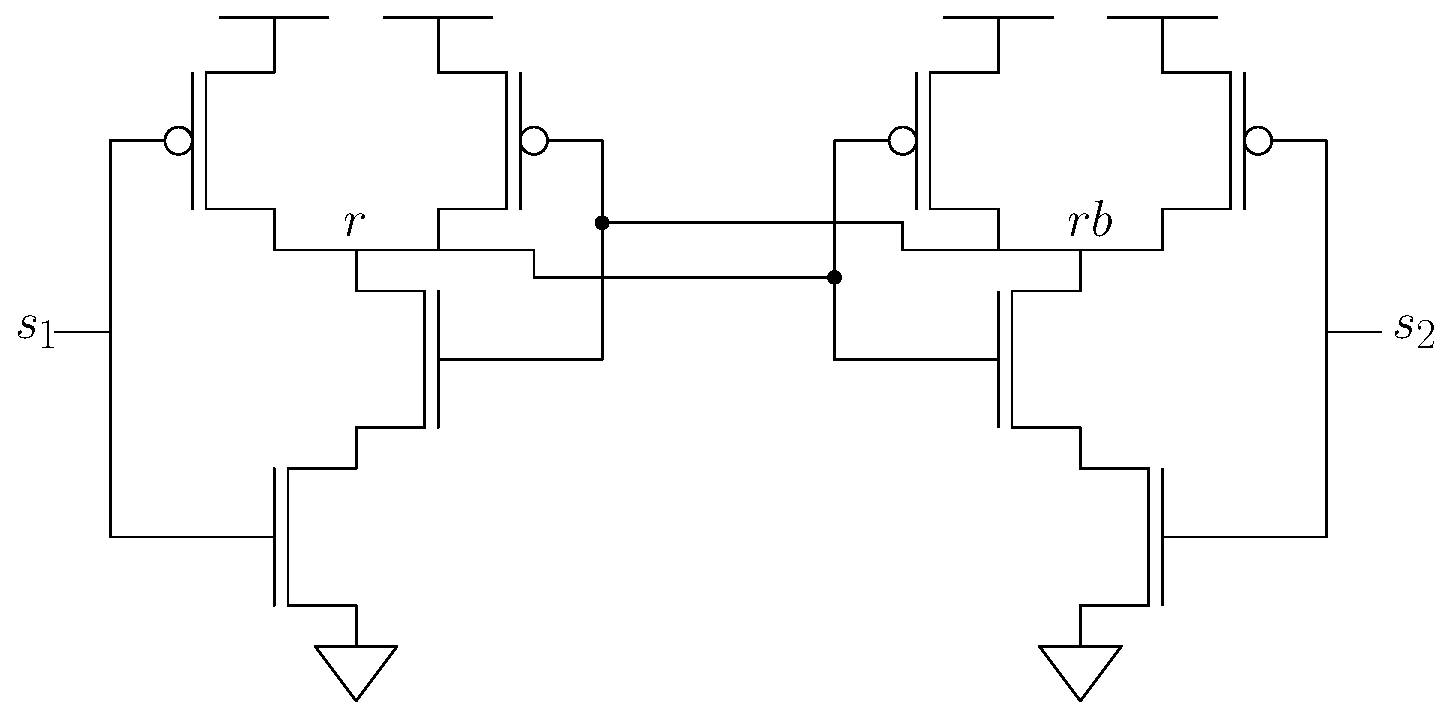
\includegraphics[width=0.80\textwidth]{images/arbiter_circuit.eps}
% \noindent\includegraphics[width=1.00\textwidth, height=3cm, draft]{example-image-a}
%\cite{Lin2010Low-powerFunctions}
% https://en.wikipedia.org/wiki/NAND_gate
\caption[Arbiter circuit]{Arbiter switching circuit realized with \ac{CMOS} NAND gates. The outputs $r$ and $rb$ start with the initial state high. If signal $\gls{s}_1$ appears first, the output $r$ will change to low, whereas $rb$ stays high. If signal $\gls{s}_2$ arrives first, it will behave the other way round.}
\label{fig:nandarbiter}
\end{figure}

All presented \apuf \ac{ASIC} implementation properties are considered when creating the \apuf simulation in Sec.\ \ref{sec:pufsimulation}.
This work does not examine physical \apuf implementations further, since they are not needed for understanding of \ac{ML} attacks.

%========================================

\subsection{Theoretical}
\label{sec:theoretical}

Every \apuf can be exactly represented by a theoretical model when all delay difference values of all stages and the noise distribution attributes are known.
This section introduces the \apuf models needed for the simulation and the attack on them.

So far the challenge space consists of the values $0$ and $1$.
For clearer notations and easier understanding that the challenge bit 1 flips the signal paths the challenge space will be converted from $\{0, 1\}^n$ to $\{-1, 1\}^n$ for the following equations.
This can be done by $p(c_i) = (-1)^{c_i}$, which means 0 becomes 1 and 1 becomes -1.

% To evaluate the response of a challenge with a specific \puf representation the sum of all delay differences chosen according to this challenge $\Delta D_{\mathrm{Model}}(c)$ and the noise values $\Delta D_{\mathrm{Noise Stage}}$ and $\Delta D_{\mathrm{Noise Arbiter}}$ is made up.
% The final response $\gls{r}$ is then calculated by the signum function of the sum:
To evaluate the response $\gls{r}$ of a challenge $\gls{c}$ of a specific \puf the sum of $\Delta D_{\mathrm{Model}}(c)$ and the noise values $\Delta D_{\mathrm{Noise Stage}}$ and $\Delta D_{\mathrm{Noise Arbiter}}$ are computed.
% Whereas the \apuf model $\Delta D_{\mathrm{Model}}(c)$ is the sum of the delay differences that are chosen depending on the challenge $\gls{c}$.
The final response $\gls{r}$ is then calculated by the signum function of the sum:

\begin{align}
r &= \operatorname{sgn}(\Delta D_{\mathrm{Model}}(c) + \Delta D_{\mathrm{Noise Stage}} + \Delta D_{\mathrm{Noise Arbiter}}). \label{equ:pufresponse}
\end{align}

The model $\Delta D_{\mathrm{Model}}(c)$, which is the noise free \apuf representation, is the sum of all delay differences that are chosen to accord with the current challenge $\gls{c}$.
% As the signal propagates though every stage after another each delay difference of the sum depends on all following challenge bits including its own.
The sign of delay difference of every stage in the sum depends on the challenge bit of the current stage and all following stages. %+
The current stage and every following stage could swap the signals and change the final response.

% Nils: proof by example?
This is easier to understand by imagine an \apuf with just two stages where the delay difference values of the second stage are 0. %+ 
% old:
% The sign of the delay difference sum is still definite by the challenge bit of the first and second stage, as the second challenge bit can always flip its stages paths or not.
The sign of the delay difference sum will be still definite by the challenge bit of the first and second stage.
The second stage, according to its challenge bit, can always flip its stages paths independently of its delay difference values.
A noise free \apuf model is thus be specified by

\begin{align}
\Delta D_{\mathrm{Model}}(c) &= \sum_{i=1}^{n}\left(\delta_{c_{i}}^{(i)}\prod_{j=i}^{n}c_{j}\right), \label{equ:pufmodelc}
\end{align}

for delay differences $\delta_{c_{i}}^{(i)}$ chosen by the bit of the challenge $c = (c_1, c_2, \cdots, c_n) \in \{-1, 1\}^n$ in the $i$-th stage of $\gls{n}$ stages.

As there are deviations in every component of the \puf when evaluating, noise needs to be modeled as well.
Noise that occurs at the arbiter $\Delta D_{\mathrm{Noise Arbiter}}$ can be modeled as a randomly drawn value of a normal distribution with zero mean and given variance $\sigmaANoise^2$ depending only on the used electronic component. %+
% While the variance of the normal distribution where the value for the total stage noise $\Delta D_{\mathrm{Noise Stage}}$ is chosen of depends beside the used electronic component on the number of stages of the \apuf as their particular noise value distributions add up.
It is a common approach to use normally distributed random values for the path delay values and all noise values \cite{Delvaux2013SideNoise,Ganji2015WhyPUFs,Ruhrmair2010ModelingFunctions}.

Noise that occurs at every path in every stage of the \apuf can be jointly drawn from a single normal distribution.
This normal distribution has mean zero and variance scaling relative to the number of stages of the \apuf, as the sum of normally distributed stage noise is normally distributed itself.
For that reason its random value is 

\begin{align}
\Delta D_{\mathrm{Noise Stage}} \sim \mathcal{N} (m,\ \sqrt[]{n}\ \sigmaSNoise), \label{equ:stagenoisedistribution}
\end{align}

with mean $m = 0$ and variance $\sigma_{Stage Noise}^2$ per stage for $\gls{n}$ stages.
Its standard deviation per stage adds up to the standard deviation of all stages $\sigmaASNoise$ of the \puf as follows:

% Backup:
% \begin{align*}
% \sigmaASNoise = \sqrt[]{\sigmaASNoise^2} = \sqrt[]{n \cdot \sigmaSNoise^2} = \sqrt[]{n} \cdot \sqrt[]{\sigmaSNoise^2} = \sqrt[]{n} \cdot \sigmaSNoise.
% % http://www.matheboard.de/archive/502880/thread.html
% \end{align*}
\begin{align*}
\sigmaASNoise &= \sqrt[]{\sigmaASNoise^2}\\ 
&= \sqrt[]{n \cdot \sigmaSNoise^2}\\
&= \sqrt[]{n} \cdot \sqrt[]{\sigmaSNoise^2} = \sqrt[]{n} \cdot \sigmaSNoise.
% http://www.matheboard.de/archive/502880/thread.html
\end{align*}

The introduced noise leads to unstable challenges, as explained in Sec.\ \ref{sec:arbiter}.
To define these unstable challenges precisely, we define the stability $\Stab(\gls{c})$ for challenge $\gls{c}$ to be

\begin{align}
\Pr[\operatorname{sgn}(\Delta D_{\mathrm{Model}}(c) + \Delta D_{\mathrm{Noise Stage}} + \Delta D_{\mathrm{Noise Arbiter}}) = \operatorname{sgn}(\Delta D_{\mathrm{Model}}(c))]. \label{equ:stability}
\end{align}

% Within all these parts to completely model an \apuf the noise free model $\Delta D_{\mathrm{Model}}(c)$ is the part with the intrinsic key which want to be attacked.
For a realistic model of an \apuf, noise has to added, as described. 
However, the noise free model $\Delta D_{\mathrm{Model}}(c)$ is the part with the hidden information, which an attacker want to expose. %+
As widely common and used in attacks on \apuf, the noise free model can be specified in a case-distinction-free form and as linear function of dimension $\gls{n} + 1$ also called linear threshold function \cite{Majzoobi2008TestingSecurity, Majzoobi2008LightweightPUFs, Ruhrmair2010ModelingFunctions, Becker2015ThePUFs, Gassend2004IdentificationCircuits, Ganji2016PACPUFs}.
An equal representation is used in this work to attack different types of \apufs.
The function is definite by

\begin{align}
\Delta D_{\mathrm{Model}}(x) &= \sum_{i=0}^{n+1} w_i x_i = \langle w,x\rangle, \label{equ:pufmodelw}
\end{align}

whereas delay vector $w_i = (w_1, \cdots, w_{n+1})$ includes the delay differences $\delta_{c_i}^{(i)}$ of all stages and is calculated as follows:

\begin{align*}
w_1 &= \delta_{0}^{(1)} - \delta_{1}^{(1)},\\
w_i &= \delta_{0}^{(i-1)} + \delta_{1}^{(i-1)} + \delta_{0}^{(i)} - \delta_{1}^{(i)}\ \text{for}\ 2 \le i \le n,\\
w_{n+1} &= \delta_{0}^{(n)} + \delta_{1}^{(n)}.
\end{align*}
 
The feature vector $\gls{x}$ is computed from the challenge $\gls{c}$ by

\begin{equation}
\begin{aligned}
x_i &= \prod_{i=1}^n c_i,\\ 
x_{n+1} &= 1. \label{equ:featurevector}
\end{aligned}
\end{equation}

As in Sec.\ \ref{sec:xorarbiterpufs} introduced, \xpufs include $\gls{k}$ multiple \apufs whose single responses are combined by a \ac{XOR} function to the final response.
% The \ac{XOR} function is represented by an multiplication hence equation
The \ac{XOR} function is represented by multiplication in the $\{-1,1\}^n$ challenge space.
Hence, we can model the response $\gls{r}$ of a \xpuf by

\begin{align*}
r &= \prod_{i=1}^k \operatorname{sgn}(\Delta D_{\mathrm{Model}}^i(x)) = \prod_{i=1}^k \operatorname{sgn}(\langle w_i,x\rangle)
\end{align*}

for the noise free \xpuf model.
Since the challenge $\gls{c}$ is the same for all \apufs, the feature vector $\gls{x}$ stays the same as well.
The feature vector is applied to all \apufs and only the \apuf model $\gls{w}$ changes. %+
Here introduced models are used in both to simulate attackable \apuf instances in Sec.\ \ref{sec:pufsimulation} and in the attacks on them in Sec.\ \ref{sec:machinelearningdesign}.

%========================================


%========================================
%========================================
% Moved to new chapter 6 Attacks
% Backup:

% \section{Attacks on \apufs}
% \label{sec:attacksonarbiter}

% Since \apufs were one of the most promising \puf implementation multiple attacks have been developed.
% One of the first attacks reveals the internal values of the \apuf by linear programming \cite{Ozturk2008TowardsDevices}.
% This approach solves a linear equation system after collecting enough \acp{CRP} because an \apuf can be represented as linear threshold function, as shown in Sec.\ \ref{sec:theoretical}.
% For a good result the stability of the responses of the \acp{CRP} should be as high as possible.
% As the response of every \ac{CRP} includes some noise as explained in Sec.\ \ref{sec:physical} one strategy of the attacker is to reduce the noise by using majority vote, i.e. evaluating the same challenge multiple times and picking the most appeared response.
% Therefor the attacker has to be able to evaluate chosen challenges.
% Another option would be using an algorithm to learn noisy linear threshold function as Blum et al.\ showed can be done in polynomial time \cite{Blum1998AlgorithmicaNoisy}.

% The linear programming attack is a non-invasive modeling attack where the attacker needs to collect \acp{CRP} to build a model of the \puf by for example a \ac{ML} algorithm.
% After that the model can predict responses for new challenges which have not be used to create the model itself.
% How precise these predictions are depends on the number of captured \acp{CRP} and which parameters have been used to build the model.
% The result and the model building performance vary for different \ac{ML} techniques.
% How the attacker gets to know the \acp{CRP} in a real use case depends on the way the \puf is used and the \acp{CRP} transmitted and therefore not part of this work.
% As \apufs are strong \pufs and their operation frequency is relatively high they provide the option to freely access a large amount of \acp{CRP} \cite{Ruhrmair2010ModelingFunctions}.
% On the contrary some \pufs post-process their response in the protected chip environment to make the \puf response itself inaccessible to protect the \puf \cite{Suh2007PhysicalGeneration, Gassend2004IdentificationCircuits}.
% All non-invasive attacks mentioned in this thesis investigate \pufs despite how they obtain \acp{CRP}.
% For this reason I assume to have free access to the \puf and be able to measure \acp{CRP} without restrictions.
% % difference machine learning to algebraic technique like linear programming \cite{Ruhrmair2014PUFOverview} Page 1

% It has been shown by Rührmair et al.\ that \apufs can be successfully attacked resulting in a model with even higher stability as the \apuf in-silicon implementation has \cite{Ruhrmair2010ModelingFunctions}.
% For these attacks he used \acp{SVM}, \ac{LR}, and \ac{ES} where \ac{LR} performed best in terms of predicting randomly chosen challenges.
% Other techniques to create accurate \apuf models are \ac{ANN} and \ac{PAC} learning whereas \ac{PAC} is an analysis algorithm and not a \ac{ML} technique. 
% \acp{ANN} need a relative large amount of \acp{CRP} to achieve a high prediction accuracy of new challenges \cite{Hospodar2012MachineUsability}.
% The approach for a \ac{PAC} learning algorithm by Ganji et al.\ requires an \ac{DFA} based representation of \apufs to attack them successfully \cite{Ganji2016PACPUFs}.
% A further attack is the reliability-based machine learning attack by Becker \cite{Becker2015ThePUFs}.
% It is based on the reliability of the \puf responses rather than on their values. 
% This in combination with an \ac{CMA-ES} algorithm makes it possible to create \apuf model with high accuracy.

% Beside these non-invasive modeling attacks are side channel attack possible.
% As mentioned before, in real attack scenarios, the \puf response or a large set of \acp{CRP} is may be not available to the attacker so he has to obtain information differently.
% As an example the photonic emission analysis attack where the attacker measures the evolved photons of the bottom side of the \apuf chip to reveal all its internal delay values \cite{Tajik2014PhysicalPUFs}.
% With these values the attacker can create an exact model of the \apuf as explained in Sec.\ \ref{sec:theoretical}.
% Different combinations of machine learning attacks and side channel attacks have been proposed as well \cite{Mahmoud2013CombinedPUFs, Xu2014Hybrid}.
% However, in this work I focus only on non-invasive machine learning attacks as they do not require physical access to the \apuf chip.

% %========================================

% \section{Attacks on \acs{XOR} \apufs}
% \label{sec:attacksonxorarbiter}

% Many attacks on \apufs can also be applied to \xpufs.
% As main differences the attacks additionally have to cope with the added non-linearity by the \ac{XOR} function, the increasing number of \apufs, and the fact that the responses of all \apufs are not individually accessible.
% The increasing number of \apufs make the time consumed by the attack and its growth rate an important factor for building secure \xpufs that can not be successfully modeled in reasonable time.
% On the one hand, this time grows with the number of used \apufs for the most attacks exponentially and on the other hand, the size $\gls{k}$ of a \xpuf is limited by the growing total noise as explained in Sec.\ \ref{sec:xorarbiterpufs} \cite{Ruhrmair2010ModelingFunctions}.
% The reports about current effective attacks on \xpufs differ in the maximum size $\gls{k}$ by $4$ to $6$ \cite{Ganji2015WhyPUFs, Xu2014Hybrid}.
% Under these conditions Ganji et al.\ developed a \ac{PAC} learning algorithm to successfully model \xpufs \cite{Ganji2015WhyPUFs}.
% Using \ac{ANN} and \ac{SVM} proved to be rather inefficient when $\gls{k} > 2$ \cite{Hospodar2012MachineUsability}.
% Equally bad performed the \ac{ES} attack.
% However, the \ac{LR} algorithm is able to model \xpufs of size $k \le 6$ by $n = 64$ \cite{Ruhrmair2010ModelingFunctions}.
% All attacks mentioned so far grow exponentially in their execution time for linear increasing $k$.
% \todo{Nils:a comparison table would be great}
% Only the \ac{CMA-ES} attack that is based on the reliability of the responses claims to have linear growing time consumption for rising $k$ \cite{Becker2015ThePUFs}.
% That means for example using double the amount of \apufs in a \xpufs leads only to twice the required time to run this attack.

% %========================================





